% -*- TeX:de -*-
\NeedsTeXFormat{LaTeX2e}
\documentclass[12pt,a4paper,titlepage]{article}

%\usepackage[german]{babel} % german text
\usepackage[DIV12]{typearea} % size of printable area
\usepackage[T1]{fontenc} % font encoding
\usepackage[utf8]{inputenc} % probably on Linux

\usepackage{graphicx} % to include images
\graphicspath{ {img/} } % set default image directory
\usepackage{subfigure} % for creating subfigures
\usepackage{amsmath} % a bunch of symbols
\usepackage{amssymb} % even more symbols
\usepackage{booktabs} % pretty tables
\usepackage{csquotes}

% a floating environment for circuits
\usepackage{float}
\usepackage{caption}

\newfloat{circuit}{tbph}{circuits}
\floatname{circuit}{Schaltplan}

% a floating environment for diagrams
\newfloat{diagram}{tbph}{diagrams}
\floatname{diagram}{Diagramm}

\renewcommand{\familydefault}{\sfdefault} % activate to use sans-serif font as default

\sloppy % friendly typesetting

\usepackage{eurosym}
\usepackage{makeidx}
\usepackage{amsfonts}
\usepackage{mparhack}
\usepackage{array}
\usepackage{tabularx}
\usepackage{minitoc}
\usepackage[colorlinks=true]{hyperref}
\usepackage{epstopdf}
\usepackage{setspace}
\usepackage{csquotes}

% hyperref settings
\hypersetup{
    colorlinks=false,       % false: boxed links; true: colored links
    linkcolor=black,          % color of internal links (change box color with linkbordercolor)
    citecolor=black,        % color of links to bibliography
    filecolor=black,      % color of file links
    urlcolor=black           % color of external links
}

\begin{document}

\begin{titlepage}

\begin{figure*}[h!]
  
\includegraphics[width=8cm]{TULogo_CMYK}
\end{figure*}

\begin{center}
\vspace*{1.3cm}
{\Huge Elektrotechnische Grundlagen der Informatik\\(LU 182.692)\\}
\vspace{1.7cm}
{\LARGE Protokoll der 2. Labor\"ubung: \enquote{Filter}\\}
{\large \enquote{Transiente Vorg\"ange und Frequenzverhalten}\\}
{\LARGE b) Messungen\\}
\vspace{1.5cm}

% fill in group number and date of lab here
% CHANGE ME!
{\Large Gruppennr.: 22 \hspace{1cm} Datum der Labor\"ubung: 19.05.2017}

% fill in IDs and names here
% CHANGE ME!
\begin{table}[h!]
\centering
\begin{tabular}{|p{3.5cm}|p{3.5cm}|p{6.5cm}|}
\hline \textbf{Matr. Nr.} & \textbf{Kennzahl} & \textbf{Name} \\
\hline
1614835 & 033 535 & Jan Nausner \\
\hline
1633068 & 033 535 & David Pernerstorfer \\
\hline
\end{tabular}
\end{table}

\end{center}
\vspace{1.0cm}

\begin{table}[h!]
\begin{tabular}{|l|l|}
\hline \textbf{Kontrolle} & \checkmark \\
\hline Verhalten eines Filters 1. Ordnung & \\
\hline Verhalten eines RL-Filters & \\
\hline Dynamisches System 2. Ordnung & \\
\hline
\end{tabular}
\end{table}

\end{titlepage}
% start of actual lab protocol
% CHANGE ME!

\setcounter{page}{2}

\newpage
\setcounter{tocdepth}{1}
\tableofcontents

\newpage

\section*{Materialien}
\begin{itemize}
	\item Oszilloskop: Agilent InfiniiVision MSO-X 3054A
	\item Frequenzgenerator: Agilent 33220A
  \item Multimeter: Amprobe 37XR-A
\end{itemize}

\section{Messung des Verhaltens eines RC-Filters 1. Ordnung}

\subsection{Aufgabenstellung}

\subsection{Schaltplan}

\subsection{Durchf\"uhrung}

\subsection{Ergebnis \& Diskussion}

\section{Messung des Verhaltens eines RL-Filters 1. Ordnung}

\subsection{Aufgabenstellung}

\subsection{Schaltplan}

\subsection{Durchf\"uhrung}

\subsection{Ergebnis \& Diskussion}

\section{Messung des Verhaltens eines dynamischen Systems 2. Ordnung}

\subsection{Aufgabenstellung}
Die Sprungantwort sowie das Frequenzverhalten eines RLC-Systems 2. Ordnung soll untersucht werden.

\subsection{Schaltplan}
\begin{figure}[H]
  \centering
  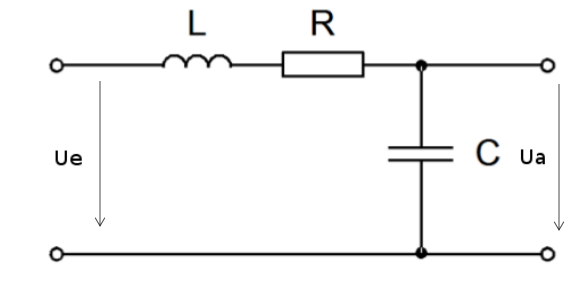
\includegraphics[width=100mm]{rlc_schaltplan.png}
  \caption{RLC-System 2.Ordnung}
\end{figure}

\subsection{Durchf\"uhrung}
Die Schaltung wurde gem\"aß Schaltplan mit den Bauteilwerten $L=1mH$, $C=100nF$ und $R=22\Omega$ aufgebaut. Um die Sprungantwort des Systems mit dem Oszilloskop aufzuzeichnen, wurde als Eingangssignal eine periodische Rechteckschwingung mit $1Vpp$, Offset $0,5V$ und Frequenz $2,5kHz$ (Periodendauer $400\mu s$) angelegt. Weiters wurde das Frequenz- bzw. D\"ampfungsverhalten des Systems mit einem Sinussignal ($1Vpp$) ermittelt. Hierbei wurde zuerst die Resonanzfrequenz durch Variation der Frequenz des Eingangssignals bestimmt. Diese ist erreicht, wenn Eingangs- und Aussgangsignal eine Phasenverschiebung von $-90^{\circ}$ zueinander aufweisen. Um den Amplitudengang des Systems zu ermitteln, wurden Eingangs- und Ausgangspannung an verschiedenen Frequenzmesspunkten im lograithmischen Maßstab ermittelt. Im Bereich der Resonanzfrequenz wurden zusätzlich Messpunkte gewählt, um die Genauigkeit zu erhöhen. Die oben beschriebene Vorgangsweise wurde mit den Widerstandswerten $R = 183 \Omega$ (in der Angabe wurden $180\Omega$ verlangt, es gibt jedoch keinen Normwiderstand mit diesem Wert, darum wurden hier ein $150\Omega$ und ein $33\Omega$ in Serie geschalten) und $R = 1k\Omega$ wiederholt.

\subsection{Ergebnis \& Diskussion}
\begin{figure}[H]
  \centering
  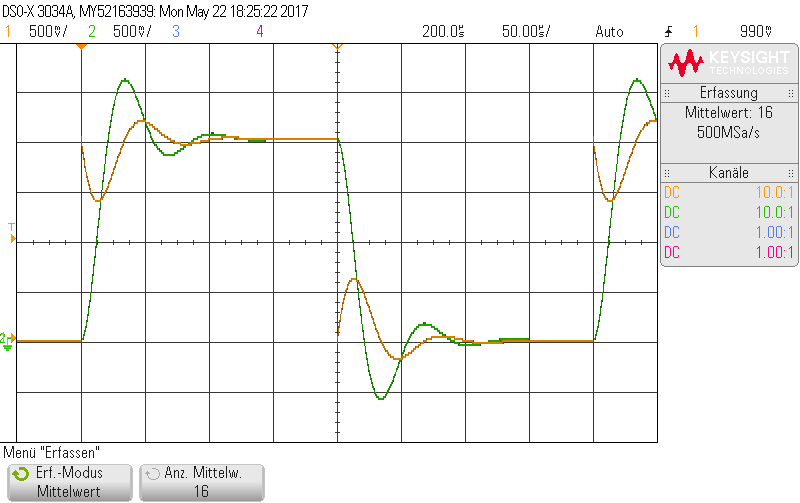
\includegraphics[width=100mm]{sprungantwort_rlc_22.png}
  \caption{Sprungantwort bei $R=22\Omega$}
\end{figure}
Durch den kleinen Widerstand ($R=22\Omega$) ist die Dämpfung des Systems sehr gering und es wird auch das Schwingungsverhalten des $LC$-Glieds deutlich sichtbar (\"Uberschwingung). Verursacht durch die parasit\"aren Eigenschaften der realen Bauelemente kommt es auch zu Reflexionen, die sich auf die Messung der Eingangsspannung auswirken.

\begin{figure}[H]
  \centering
  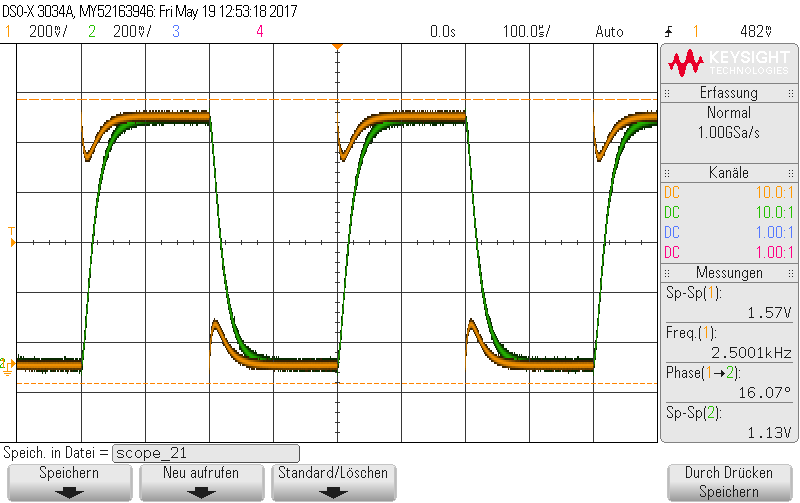
\includegraphics[width=100mm]{sprungantwort_rlc_180.png}
  \caption{Sprungantwort bei $R=183\Omega$}
\end{figure}
\noindent Bei $R=183\Omega$ sind gerade keine \"Uberschwingungen sichtbar (aperiodischer Grenzfall). Die Sprungantwort zeigt das typische Tiefpassverhalten.

\begin{figure}[H]
  \centering
  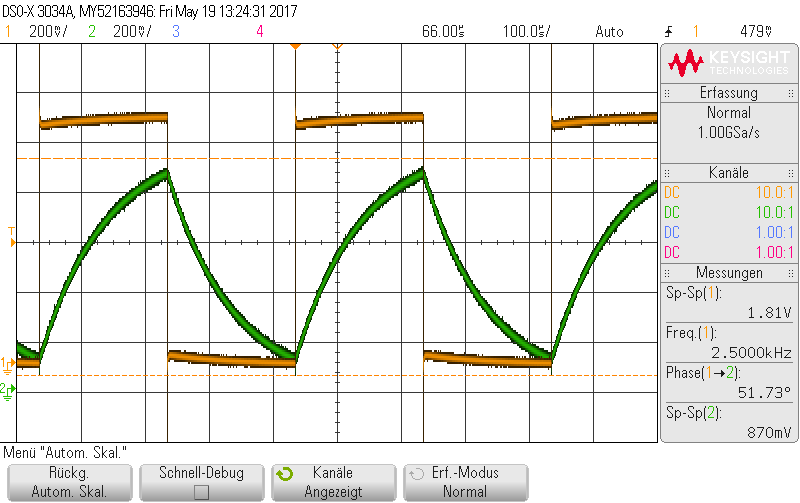
\includegraphics[width=100mm]{sprungantwort_rlc_1k.png}
  \caption{Sprungantwort bei $R=1k\Omega$}
\end{figure}
\noindent Durch den großen Widerstand von $R=1k\Omega$ wird die D\"ampfung des Systems sehr groß. Dadurch wird in der Folge die anliegende Rechteckspannung stark verschliffen (die Energiespeicher werden durch die große Zeitkonstante nie vollst\"andig geladen).\\\\
Die Resonanzfrequenz des Systems ergibt sich aus folgender Formel:
\begin{figure}[H]
  \centering
  $f_R = \sqrt{f_H*f_L} = \frac{1}{2\pi\sqrt{LC}} \approx 15916Hz$
\end{figure}

\noindent Die \"Ubertragungsfunktion des Systems lautet:
\begin{figure}[H]
  \centering
  $\frac{U_a}{U_e} = \frac{Z_C}{Z_R+Z_L+Z_C} = \frac{\frac{1}{j\omega C}}{R+j\omega L+\frac{1}{j\omega C}} = \frac{1}{j\omega CR-\omega^2CL+1} = \frac{1}{s^2CL+sCR+1}$
\end{figure}

\begin{figure}[H]
  \centering
  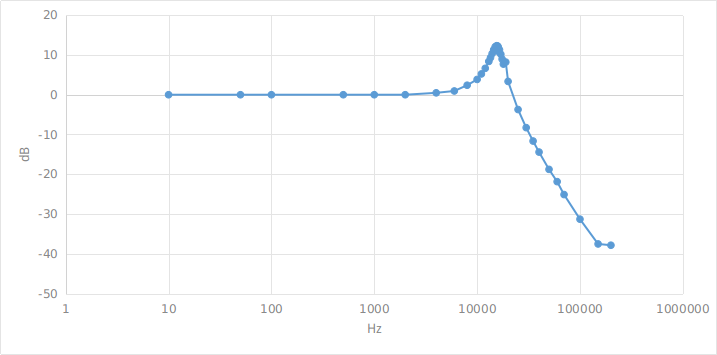
\includegraphics[width=150mm]{bode_rlc_22.png}
  \caption{Bode-Diagramm (Amplitudengang) bei $R=22\Omega$}
\end{figure}
\noindent Die gemessene Resonanzfrequenz betr\"agt hier $\sim15800Hz$. Im Bereich von $f_R$ erkennt man am Bode-Diagramm, dass hier tats\"achlich eine Verstärkung des Eingangsignals stattfindet. Dies lässt sich durch die kleine Dämpfung bei $R=22\Omega$ erkl\"aren, wodurch sich das $LC$-Glied im Resonanzfall befindet. Nach dem die Resonanzfrequenz erreicht wurde, lässt sich die typische Filtersteilheilt von $-40dB/Dekade$ gut erkennen.\\
TODO: Messdaten einfügen

\begin{figure}[H]
  \centering
  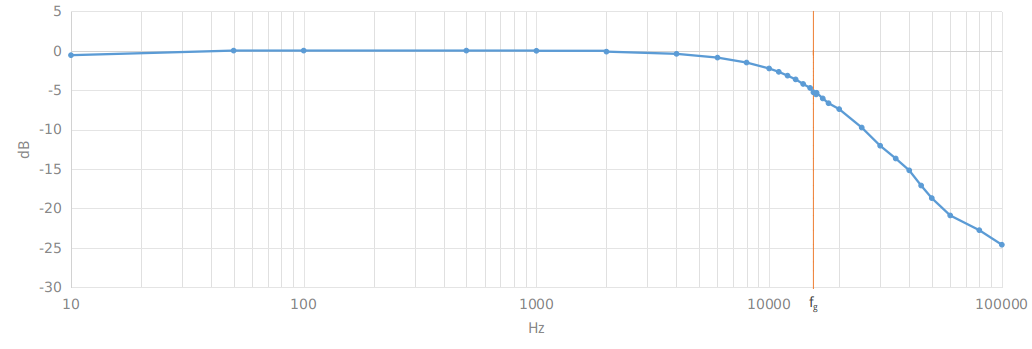
\includegraphics[width=150mm]{bode_rlc_180.png}
  \caption{Bode-Diagramm (Amplitudengang) bei $R=183\Omega$}
\end{figure}
\noindent Die gemessene Resonanzfrequenz betr\"agt hier $\sim15500Hz$. Das System befindet sich im aperiodischen Grenzfall, \\
TODO: Messdaten einfügen

\begin{figure}[H]
  \centering
  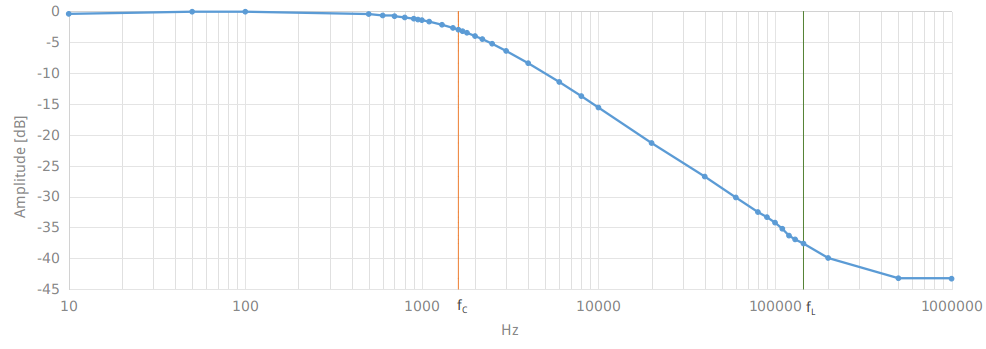
\includegraphics[width=150mm]{bode_rlc_1k.png}
  \caption{Bode-Diagramm (Amplitudengang) bei $R=1k\Omega$}
\end{figure}
TODO: Resonanzfrequenz messen\\
TODO: Messdaten einfügen\\

\begin{figure}[H]
  \centering
  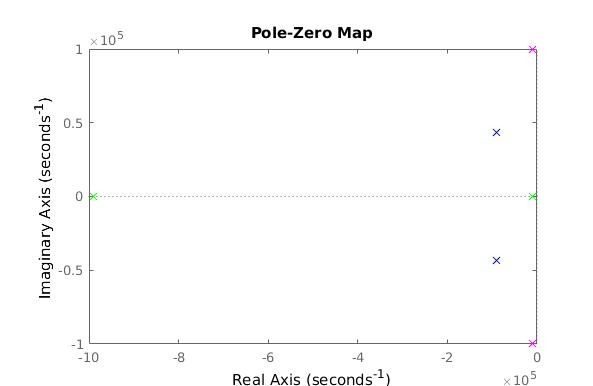
\includegraphics[width=150mm]{pnd.jpg}
  \caption{PN-Diagramm der \"Ubertragungsfunktion (violett: $R=22\Omega$, blau: $R=180\Omega$, gr\"un: $R=1k\Omega$)}
\end{figure}

\end{document}
